Projektet kändes till en början väldigt rörigt. Efter att ha arbetat med att strukturera upp projektet blev det desto tydligare. Det var mycket i projektet som kändes främmande, vilket gjorde allt aningen jobbigt, men av samma anledning var det något vi visste skulle vara väldigt lärorikt. 

Det var svårt att få en känsla av hur uppgiften skulle kunna komma till användning i praktiken, och verkade därför inte så rolig, om man jämför med ett projekt i en tidigare programmeringskurs i ML så gjorde vi ett schackspel, något som efter projektets gång tydligt visade hur bra man hade lyckats och hur det var tänkt att användas. Specifikationen för projektet kändes bra skriven till en början men ju längre projektet fortlöpte desto fler brister fann vi i den. Det saknades en hel del information som vi var tvungna att fråga om i efterhand.

Vi valde att använda oss av Git för vårt arbete. Det blev just Git för att både Niclas och Åke använt det tidigare och var mycket nöjda. Det gjorde också att det gick väldigt snabbt att komma igång med det i hela gruppen. Git gjorde det väldigt smidigt att arbeta på olika delar av programmet samtidigt. Genom att använda olika “brancher” för olika delar kan båda personer i respektive par “commita” i sin branch utan att det påverkar master-branchen, som vi hela tiden har hålt fri från inkomplett kod.

Trello är en webbbaserad tjänst där vi kunnat rita upp en “anslagstavla”. På anslagstavlan skrev vi in vad som behövdes göras, vad som är gjorts och vilka som skulle göra vad:

\begin{figure}[H]
  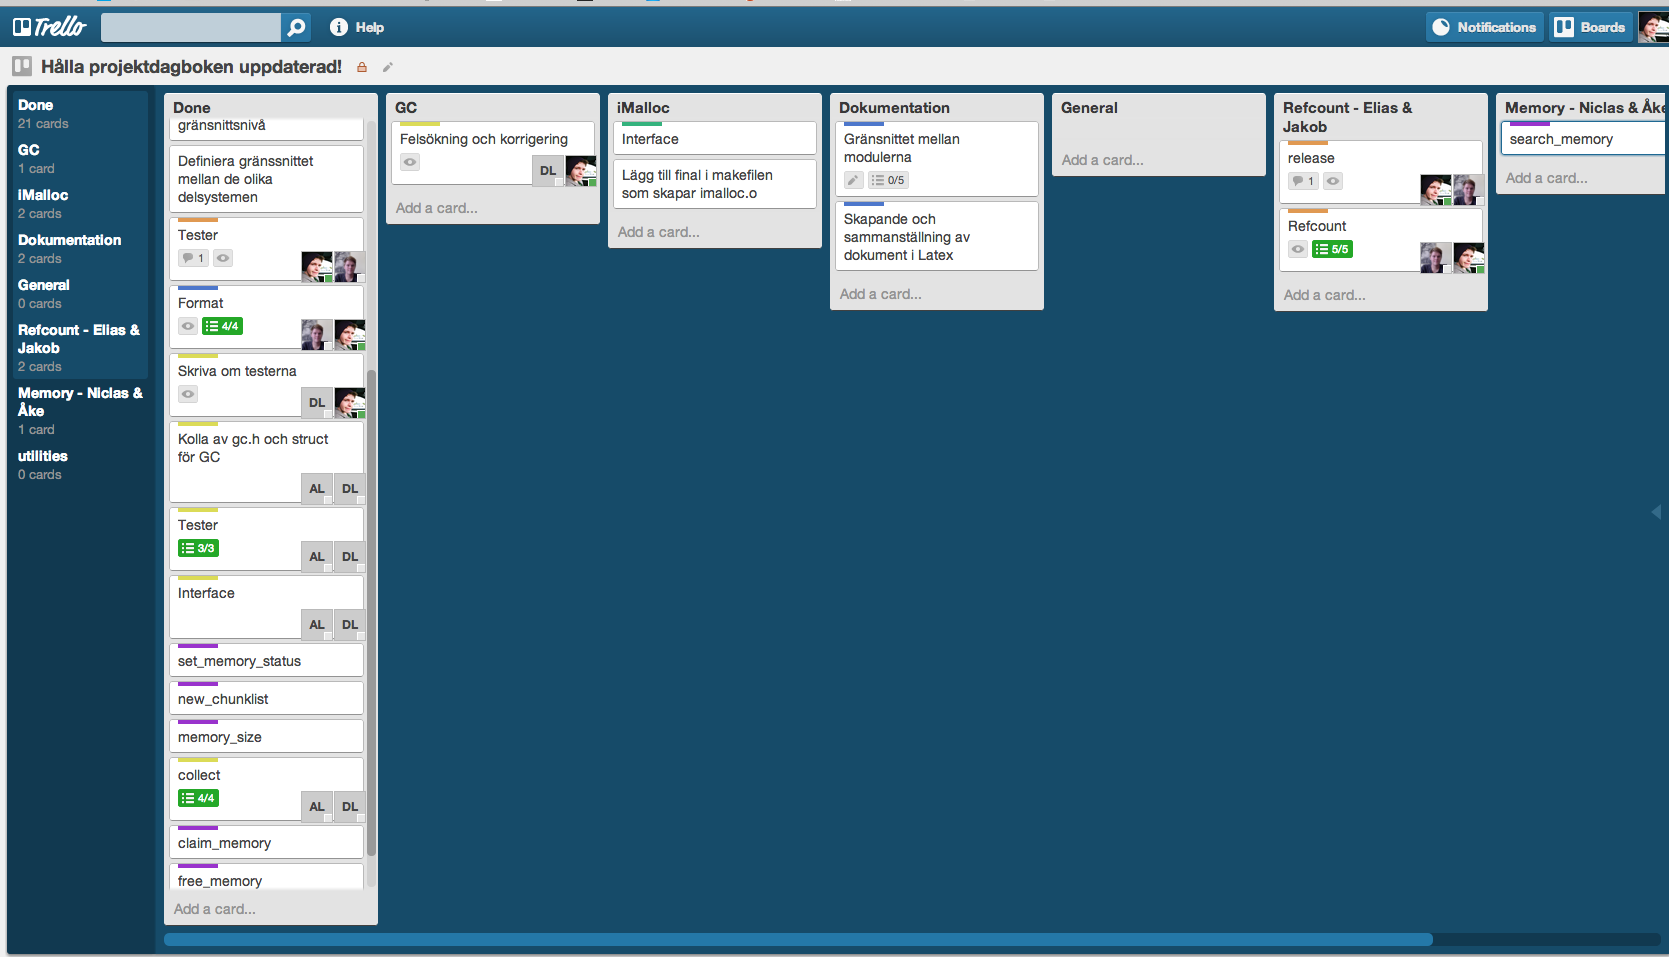
\includegraphics[width=\columnwidth]{images/trello.png}
  \caption{En skärmdump över vår trellotavla den sista veckan.}
  \label{fig:trello}
\end{figure}

Trello har varit en väldigt bra tjänst för att få översikt över projektet. Ville man jobba hemma så var det bara att se på anslagstavlan hur vi låg till och sedan arbeta vidare. Vi delade upp våra mål i små delmål som vi “bockade” av eftersom, vilket gav oss drivkraft att arbeta hårdare och fort gå vidare till nästa delmål.


Varje vardag har vi haft grupprum bokat mellan kl 8 och 17. Det har varit bra att ha som inställning och utgångspunkt - att vi ska jobba åtta timmar varje dag, ibland har någon behövt komma senare eller gå tidigare, därför har vi haft flextider. Det sista varje medlem gjorde innan de gick hem för dagen var att tidsrapportera och skriva dagbok, detta för att ständigt ha koll på vad som har blivit gjort.

I grupprummet har vi alltid haft tillgång till en whiteboard tavla, detta har vart fördelaktigt när någon har stött på problem då alla gruppmedlemmar har kunnat vara med och bolla idéer.Generellt sett har vi försökt arbeta i par så mycket det går men efter att de större delarna av programmet var klara var det svårare att dela upp arbetsuppgifterna på ett jämnt sätt, vi roterade paren trots detta men var inte rädda för att hjälpa varandra och vara lite mer flexibla i vilka uppgifter varje individ arbetade med. 

Något vi har lagt mycket vikt på under hela projektet men framför allt mot slutet var att alla skulle vara informerade av vad alla jobbade med för att således få sig en bra överblick av hur projektet fortskred. 

Diagrammen stämmer inte helt och hållet på grund av vårt sätt att jobba. Eftersom vi satt tillsammans så var ofta alla med och diskuterade fram lösningar på de problem som dök upp. De små avvikelserna tog vi inte hänsyn till när vi valde kategori att tidsrapportera till.

Tidsrapporteringen stämmer inte fullt ut då vi inte har räknat med den tid vi indirekt har arbetat med de olika programdelarna, tex. när man har hjälpt varandra, istället har vi bara i slutet av dagen rapporterat det man har arbetat med i stora drag.
